\chapter{超新星遗迹在强磁场中的演化}
\label{Mag}

\section{简介}
\label{MagIntro}

在之前对超新星遗迹的模拟中,我们都是使用银河系磁场的典型值,大约9$\mu G$
\citep{Crutcher2012,Haverkorn2015}。
然而实际上,在银河系中心的致密云块中,磁场是可以达到1$mG$的\citep{Ferriere2009}。
当然,这些云块尺度并不是很大,很多相对于SNR来说很小。
不过有一些云块呈长条状,长度甚至超过SNR尺度,当然宽度可能只在1pc的量级。
这些云块很散乱,少量存在或许不会对SNR演化起到很大影响,然而银河系中心其实是大量存在这类
云块的。
这就导致,虽然大部分区域磁场仍然很弱,但是把这些云块考虑在内,平均磁场可能很强。
我们在章节~\ref{TheoryMHD}也提到,磁场会很大程度上影响SNR演化,尤其是其中粒子加速。
可是之前对SNR的研究大多关注在银河系典型磁场中的演化,当然,这其实是比较合理的,
因为银河系大部分区域的磁场还是比较弱的。
但是银河系中心单位体积内超新星爆发概率也比其它地方要高一些,这里的SNR宇宙线加速其实可能
占据整个银河系很大比重。
当然,也有很多人进行过不是针对SNR的在强磁场中的爆发模拟,这些模拟大多是用来测试MHD程序
的性能,物理上并没有解释SNR的性质\citep{Balsara1999, Stone2009, Barnes2018}。

所以,我们认为模拟SNR在强磁场中的演化是非常有必要的,这可以帮助我们理解SNR在银河系中心
的演化,并为解释宇宙线能谱提供一个参考。
不过在我们的实际模拟中发现,强磁场中的SNR形态也是非常不一样的,这可以帮助我们理解上一
章中没有解释清楚的多壳层遗迹。
本章中,我们采用了AMR技术以方便解释更细微的SNR结构和理解磁场在SNR演化中的作用。

\section{参数和结果}
\label{MagMod}
我们主要使用的初始三维网格为64 $\times$ 64 $\times$ 64,不过使用了level为4的AMR技术,
最终网格化效果接近1024 $\times$ 1024 $\times$ 1024。
此外,使用AMR画磁场、速度等矢量比较麻烦,所以我们也做了128 $\times$ 128 $\times$ 128
的模拟,方便看一下大尺度的参数变化。
另外,因为银河系平均介质密度大约为0.5 cm$^{-3}$,而考虑致密云块后的平均密度其实不太好估算,
我们在这里暂且取10 cm$^{-3}$。
作为比较,我们分别模拟了这两个密度下的SNR演化,相对应的,要达到初始半径所需的时间分别
为1881年和693年。
其它具体参数请见~\ref{table:parameters}。

\begin{table}
  \caption{强磁场中SNR模拟参数}
  \label{table:parameters}
  \centering
  \begin{tabular}{l l l}
      \hline\hline
      参数                      & 值            & 参考文献               \\
      \hline
      超新星遗迹参数\\
      \hline
      抛射质量                    & 15.8 M$_{\odot}$ & 1\\
      爆发动能                    & 2.0$\times$ 10$^{51}$ ergs & 2, 3\\
      初始半径                    & 4 pc             &\\
      模拟起始时间                & 1881 $\&$ 693 years        & 4\\
      总模拟时间                  & 10000 years\\
      \hline
      别的参数\\
      \hline
      平均介质数密度 (n)         & 0.5 $\&$ 10 cm$^{-3}$   & 5, 6\\
      磁场强度 (B)              & 900 $\mu$G   & 7, 8\\
      平均原子权重              & 1.3              &\\
      绝热系数                  & 1.7              &\\
      \hline
  \end{tabular}\\
  ~\\
  (1)\citealt{Sukhbold2016}; (2)\citealt{Poznanski2013}; (3)\citealt{Mueller2016a}; (4)\citealt{Leahy2017a};
  (5)\citealt{Nakanishi2006}; (6)\citealt{Nakanishi2016}; (7)\citealt{Haverkorn2015}; (8)\citealt{Ferriere2009}
\end{table}

初步的模拟结果在图~\ref{fig:gc}中,只展示了y-z平面的密度分布图像。
因为直接处理数据得出的矢量图太大,在电子版文章中渲染很慢,我们在这里使用截图后转的矢量图,
部分细节在放大后可能稍有出入。
图中的彩色网格是AMR网格的集中度,越密集的地方网格越多,分辨率也就越高。
另外,图像背景处看似白色的网格其实是软件的图像渲染效果,不是真实的模拟结果。
对密度为0.5 cm$^{-3}$时4500年的图像我们去掉了网格,为了看起来更清晰。
我们发现,无论何种参数,加入强磁场的SNR在演化早期就出现了明显的非球对称演化,而更偏向
于柱对称。
而这在章节~\ref{W51C}中的模拟虽然有一些倾向,但整体还是可以看作球对称的。
另外,我们发现,无论密度高低,SNR中垂直磁场方向的壳层密度更高,而平行磁场方向的壳层密度
更低。
这一现象的起因或许可以从磁场、速度矢量图上得到线索(见图~\ref{fig:low})。
垂直于磁场方向的激波再一开始会压缩磁场,而过一段时间以后,这个方向上会产生较强的反向
激波,反而向爆发中心汇聚。
其实平行于磁场方向的激波也会产生反向激波,只是很弱罢了,这种不同方向产生的反向激波
强度不同的原因自然是磁压的不同。

我们在图~\ref{fig:beta}给出了热压、磁压比$\beta_b$的分布图,很明显垂直磁场运动的激波
会放大磁场,使得$\beta_b$变小,磁压变大,总体压强变大,更容易产生反向激波。
同时,因为磁场很强,其回复力导致最初压缩的磁场慢慢回复原样。
反向激波中的物质逐渐被回复的磁场引导沿着磁场运动,流向两端。
这样一个结果导致,SNR演化大部分的物质都向沿着磁场的两端汇聚,类似喷流的准直效果。
另外,在图~\ref{fig:beta}的右图中可以看出,SNR中最大的$\beta_b$值在1左右,而
最小的值在0.01。
与带入章节~\ref{TheoryMHD}中的方程~\ref{eqn:ratio},可得$\beta_b=1$时,
$M^2=0.5+0.4+4.4=5.3, r=1.2$。
而$\beta_b=0.01$时,$M^2 \approx 40000, r \approx 1$。
其实对这个方程,本来就有$\beta_{b,2}\to 0, r \to 1$,也就是说磁场太强的时候,上下游的
密度、速度几乎不变化。
要注意的是,这并不意味着SNR上游、下游性质一样,无法区分SNR与ISM,而是一种特殊情况。
这里的磁压因为之前的压缩已经很高,本来由激波带来的动压已经无法抵挡住磁压,也就是磁场回复
的倾向。
最终磁场会像我们在模拟中展示的那样恢复到初始状态,这个回复过程必然会产生比没有磁场时更强
的反向激波,这也就是为什么我们在模拟结果中看到磁场回复的同时,反向激波很强的原因。

此外,我们看到低密度的垂直于磁场运动的激波通常比高密度的平行于磁场运动的激波运动更快,
这个也可以用我们之前推导DSA的公式来解释。
垂直于磁场的激波被磁压影响较大,大量物质被反向激波带走,所以密度低,这个很清楚。
同时,其压缩比$r$在某一时刻相对来说更小,这意味着上下游速度的差值更小。
因为这里假设超新星球对称爆发,各个方向激波速度相同,也就是说垂直和平行的激波初始速度相同。
传播过程中,激波因为与介质相互作用而减速,逐渐趋向于上下游速度一样,最终与ISM随机运动速度
一样,从而消散。
而单位时间内减速的多少由压缩比决定,因为上游速度趋向于下游速度,压缩比小意味着上下游
速度更加相近,上游减速越慢。
这里说的上下游是以激波面静止系为基准,如果周围介质在ICRF中静止,那么上游速度就是激波面
在介质中传递的速度。
而垂直于磁场的激波,压缩比总是比较小,上游速度减速也就更慢,激波面的速度也就一直更快,正
如我们在上面几幅图中看到的现象。


\begin{figure*}
    \centering
    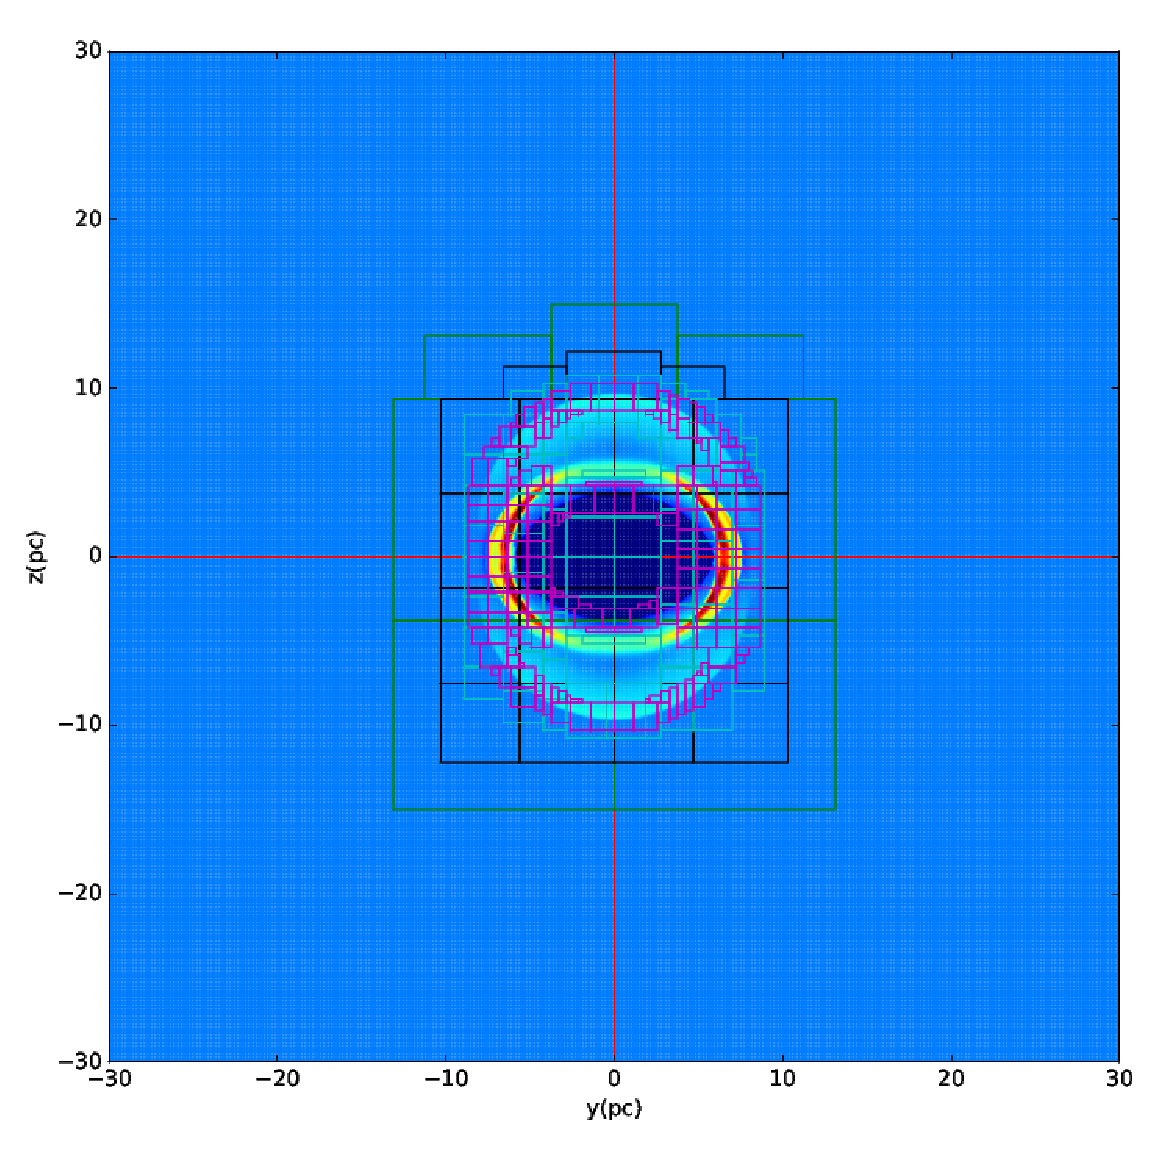
\includegraphics[width=0.455\textwidth]{1500.eps}
    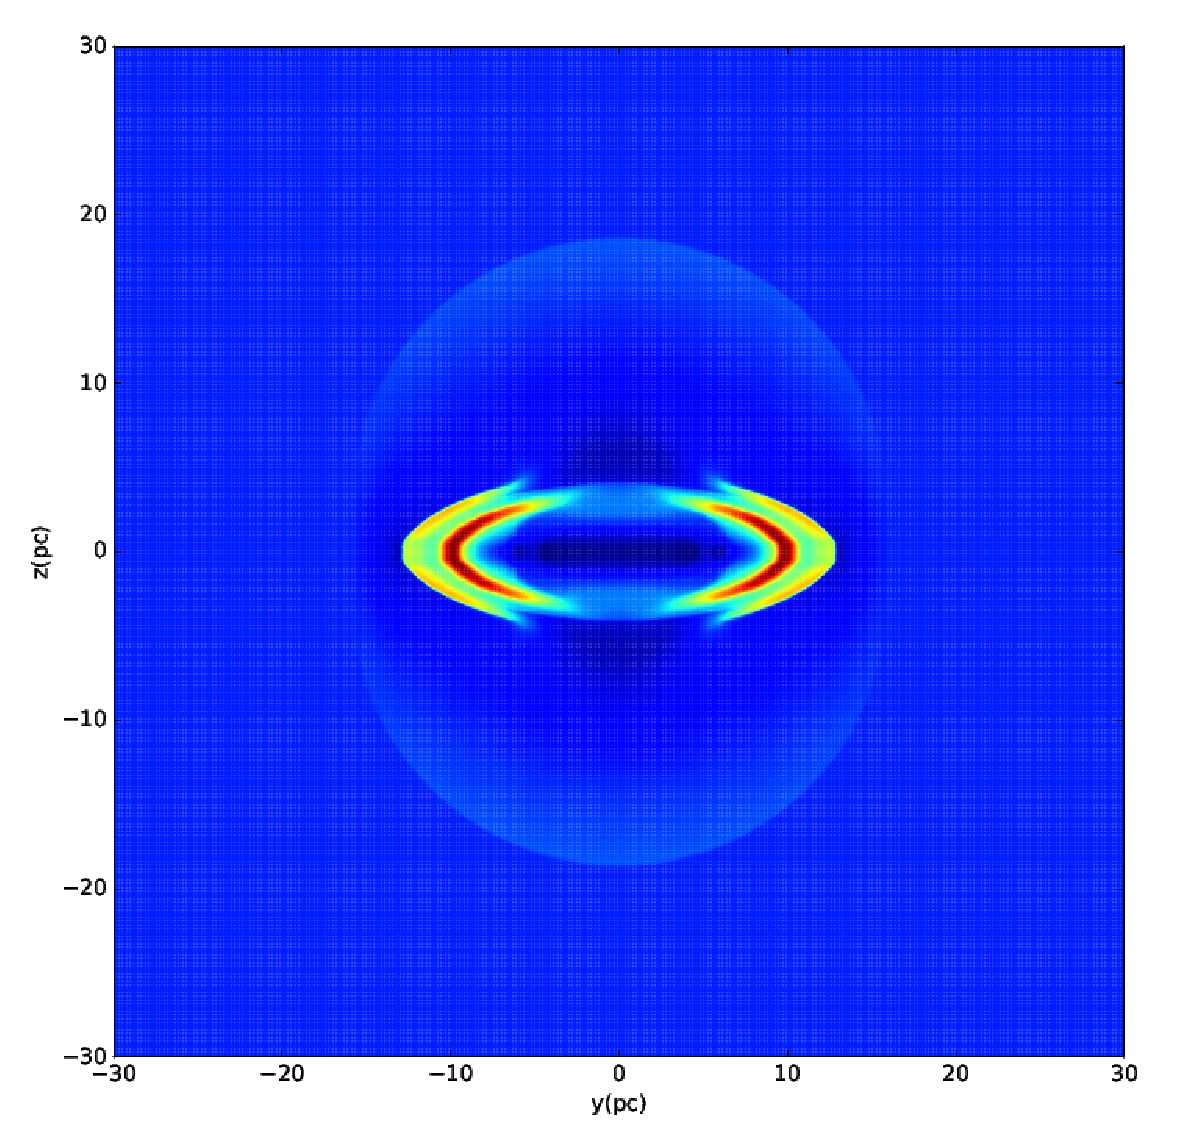
\includegraphics[width=0.455\textwidth]{4500.eps}\newline
    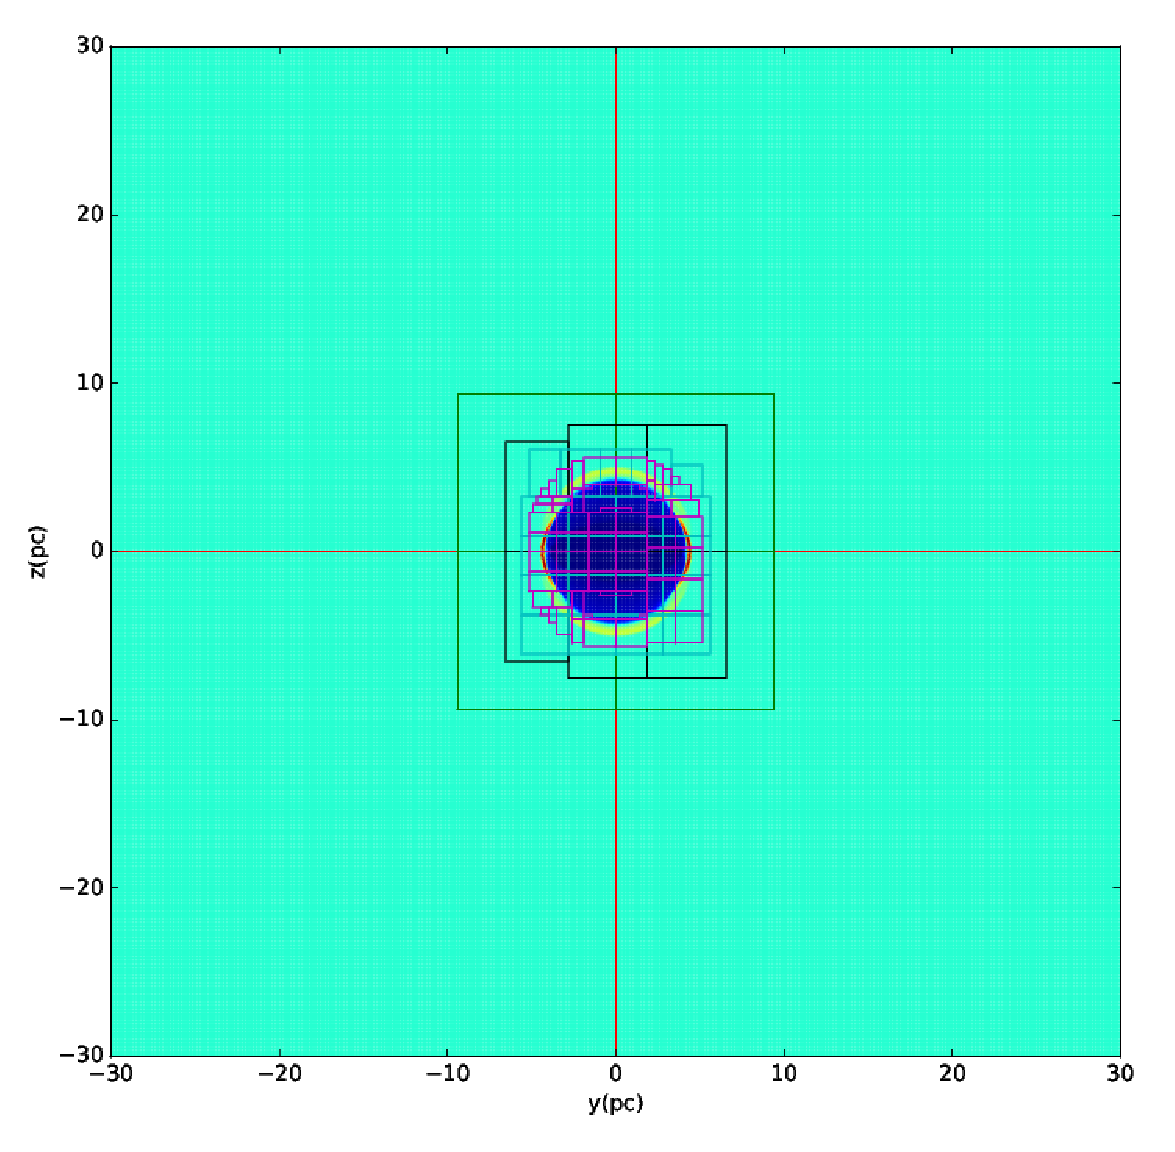
\includegraphics[width=0.455\textwidth]{1500_10.eps}
    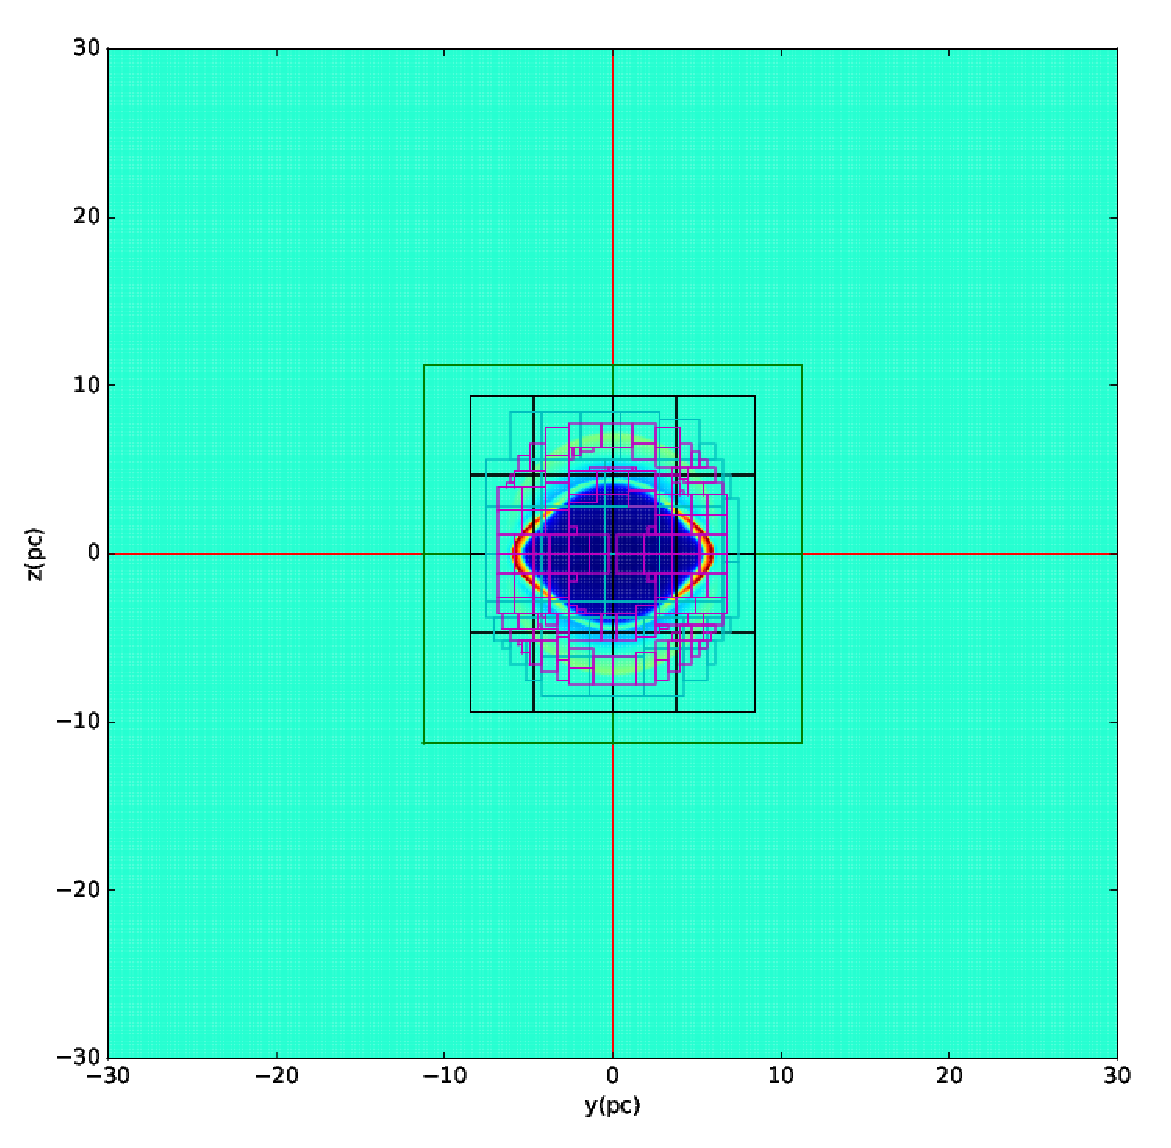
\includegraphics[width=0.455\textwidth]{4500_10.eps}
    \caption{强磁场下的高分辨率模拟的密度分布。上面两幅图是介质密度为0.5 cm$^{-3}$时
    1500年和4500年后的模拟结果。
    下面两幅图是介质密度为10 cm$^{-3}$时1500年和4500年后的模拟结果。
    上下图的真实年龄分别要再加上初始的693年和1881年。}
\label{fig:gc}
\end{figure*}

放在银河系中心考虑这件事就很有意思了。
因为银心处的磁场主要是垂直于银道面的,如果银心过去有过很多超新星爆发,那么这个准直效果
会导致很多物质在银心位置垂直于银道面抛出。
这些抛射物的初始速度至少1000 \kms ,考虑介质作用减速,千万年之后尺度也可达到kpc量级。
虽然,银心引力很强,很多物质受到引力约束,可是实际上银河系年龄也远超千万年,SNR可能
已经消散无法辨别,但是这些抛出的物质应该还可以探测到。
而最近探测到的费米泡(Fermi Bubbles)很可能也会受到这些抛射物的影响。
费米泡能谱是非热的,而最近的研究表明应该是轻子起源,有人猜测是银心黑洞在之前活动时的喷流
导致的\citep{Yang2017},可是实际上非热、轻子起源这些已知条件并不能排除SNR的贡献
\citep{Fujita2013}。

同时,这可以用来解释一些SNR射电与X射线辐射位置的差异问题。
比如SNR G1.9+0.3 \citep{Reynolds2008,Borkowski2017},这可能是银河系中最年轻的遗迹,
因为在银心附近,消光很强,所以爆发时并没有被观测到。
它的SNR射电与X射线形态与我们在这里模拟的很像,对比图~\ref{fig:low}第一张图,
在模拟图像密度高磁场小的相应位置射电辐射很强,而在模拟图像密度低磁场高的相应位置,
X射线辐射很强。
而且,我们看到,当遗迹年龄增大,这种现象会消失。
当然,我们在这里用的参数与G1.9+0.3不一样,未来还要做进一步更有针对性的模拟。

\begin{figure*}
    \centering
    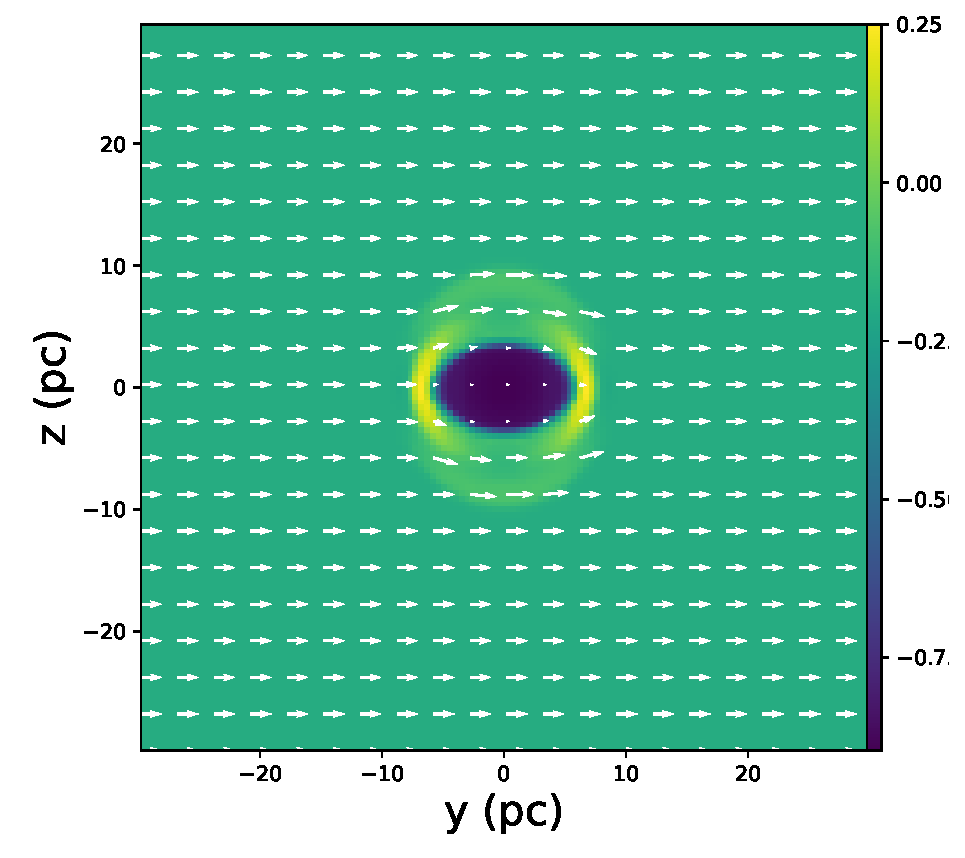
\includegraphics[width=0.455\textwidth]{rho_t3_density1_E1_yz.eps}
    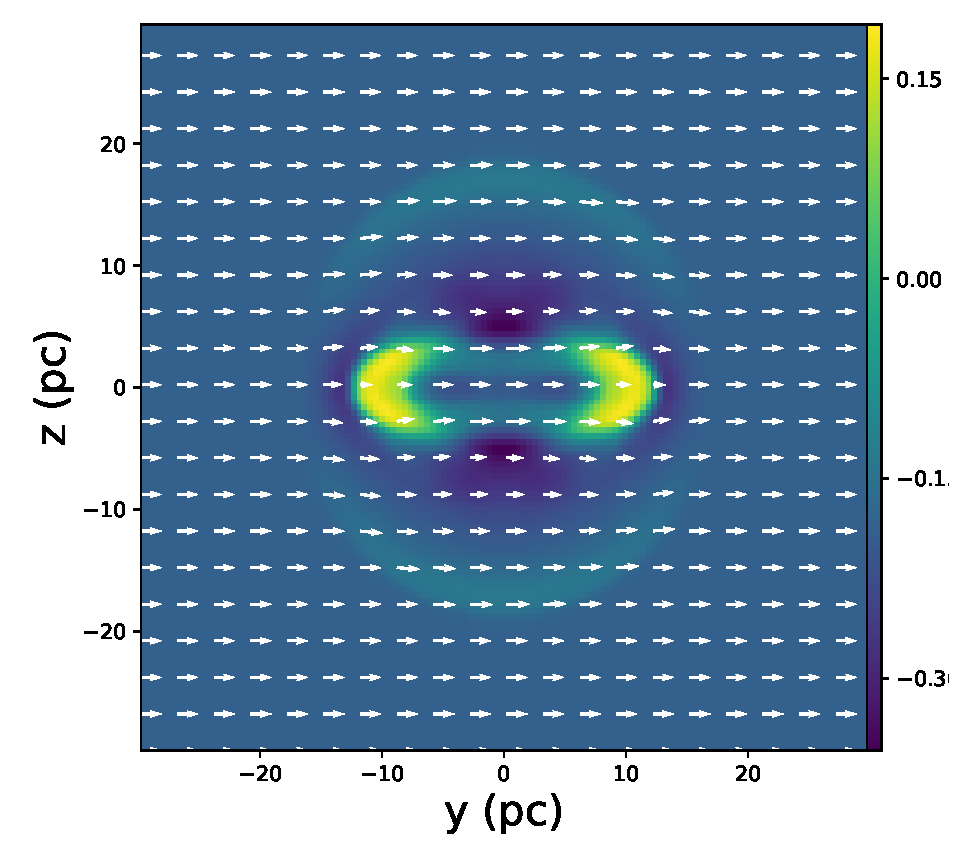
\includegraphics[width=0.455\textwidth]{rho_t9_density1_E1_yz.eps}\newline
    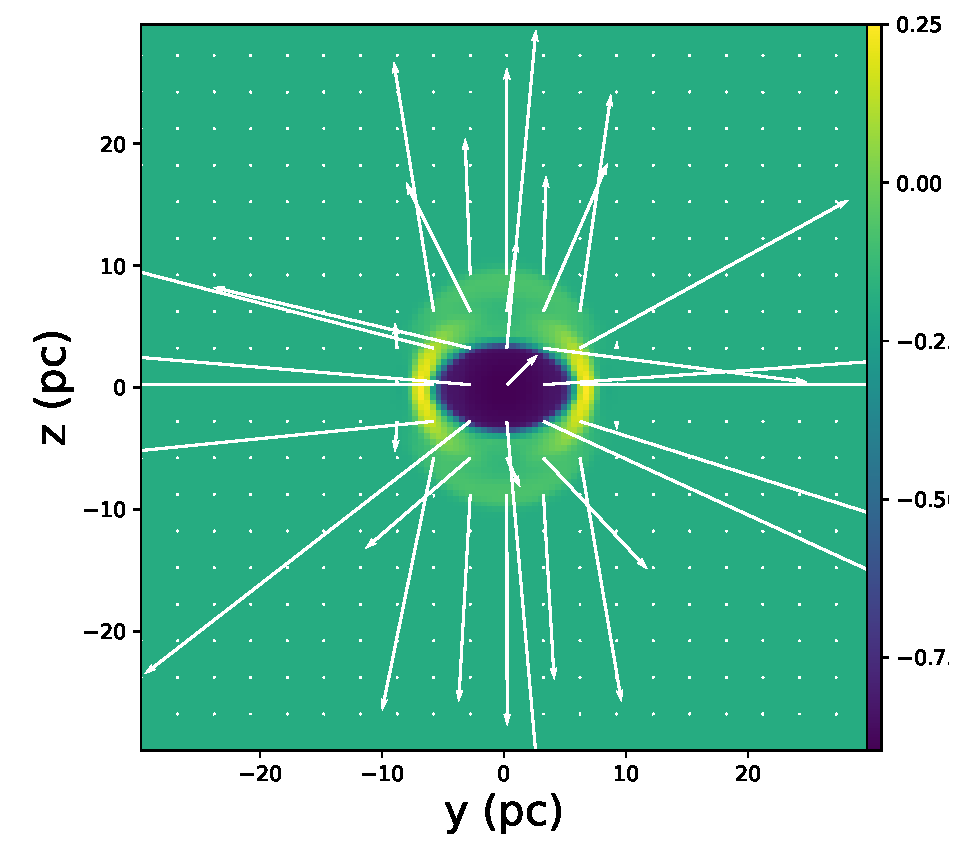
\includegraphics[width=0.455\textwidth]{rhoV_t3_density1_E1_yz.eps}
    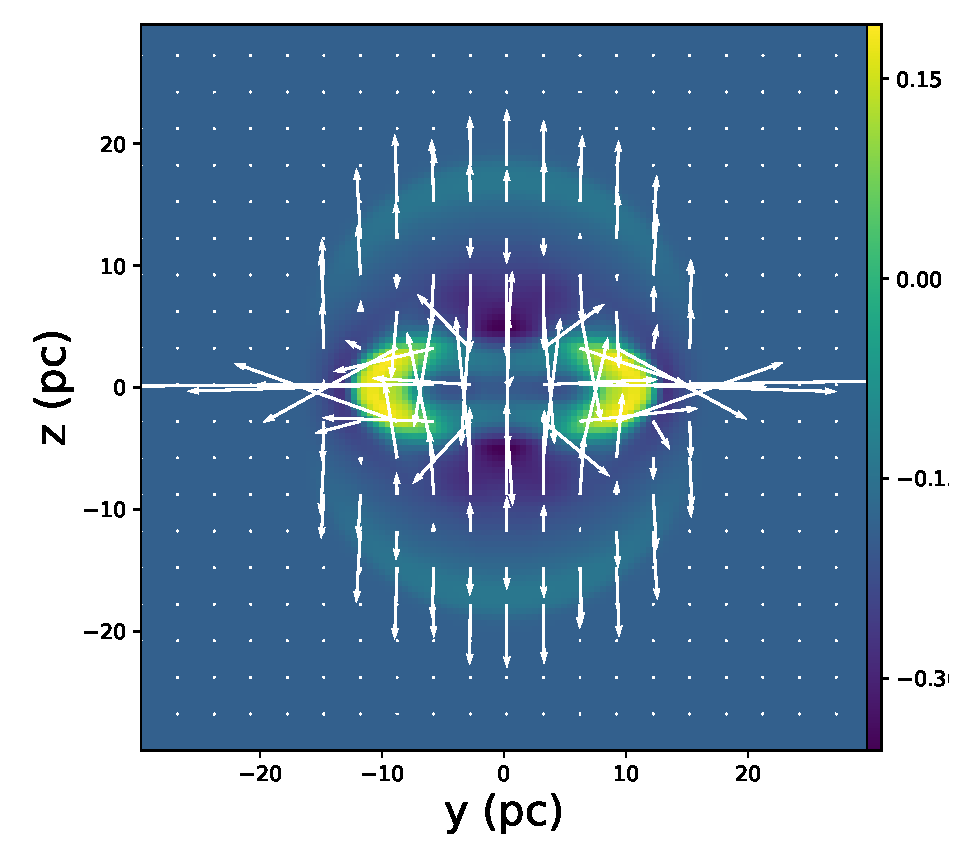
\includegraphics[width=0.455\textwidth]{rhoV_t9_density1_E1_yz.eps}
    \caption{强磁场下的低分辨率模拟的介质密度为0.5 cm$^{-3}$的模拟结果。
    上面两幅图是1500年和4500年后的密度、磁场分布,
    下面两幅图是1500年和4500年后的密度、速度分布。}
\label{fig:low}
\end{figure*}

\begin{figure*}
    \centering
    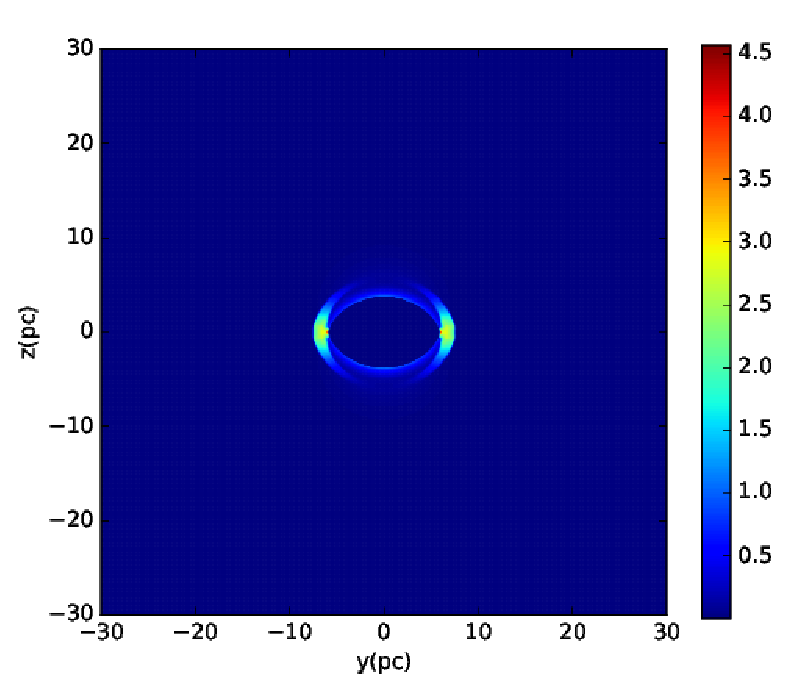
\includegraphics[width=0.455\textwidth]{1500_beta.eps}
    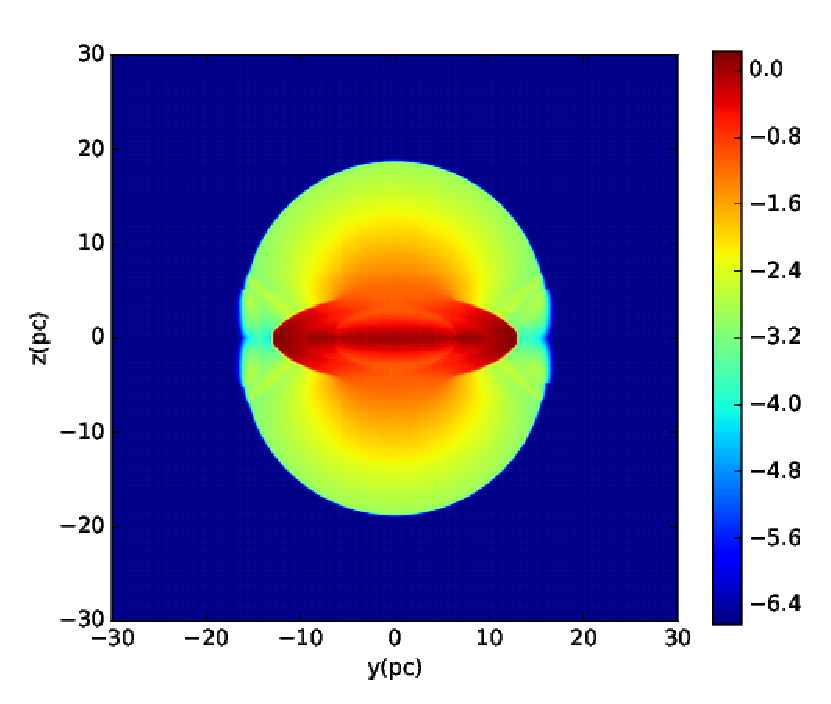
\includegraphics[width=0.455\textwidth]{4500_beta.eps}
    \caption{介质密度为0.5 cm$^{-3}$的$\beta_b$分布。
    左图是1500年后的$\beta_b$分布,右图是4500年后的$log(\beta_b)$分布。}
\label{fig:beta}
\end{figure*}

另外,我们在高分辨率的图~\ref{fig:gc}可看到,高密度区域在出现了一侧双壳层,
这可能主要是来自不同方向的反向激波与正向激波相互作用导致的,或许是章节~\ref{SW}中
多壳层遗迹的一个产生机制。
同时,我们想在这里给10 cm$^{-3}$密度下的演化10000年的结果(见图~\ref{fig:shells})。
这里的确也是出现了多壳层,但却是在相反方向。
所以,我们认为,这种多壳层的产生应该与介质密度、磁场强度、演化年龄,甚至爆发能量、
抛射物质量都有关系。
这些参数之间满足一种关系时才会产生多壳层,而目前这种关系还不明确。

\begin{figure*}
    \centering
    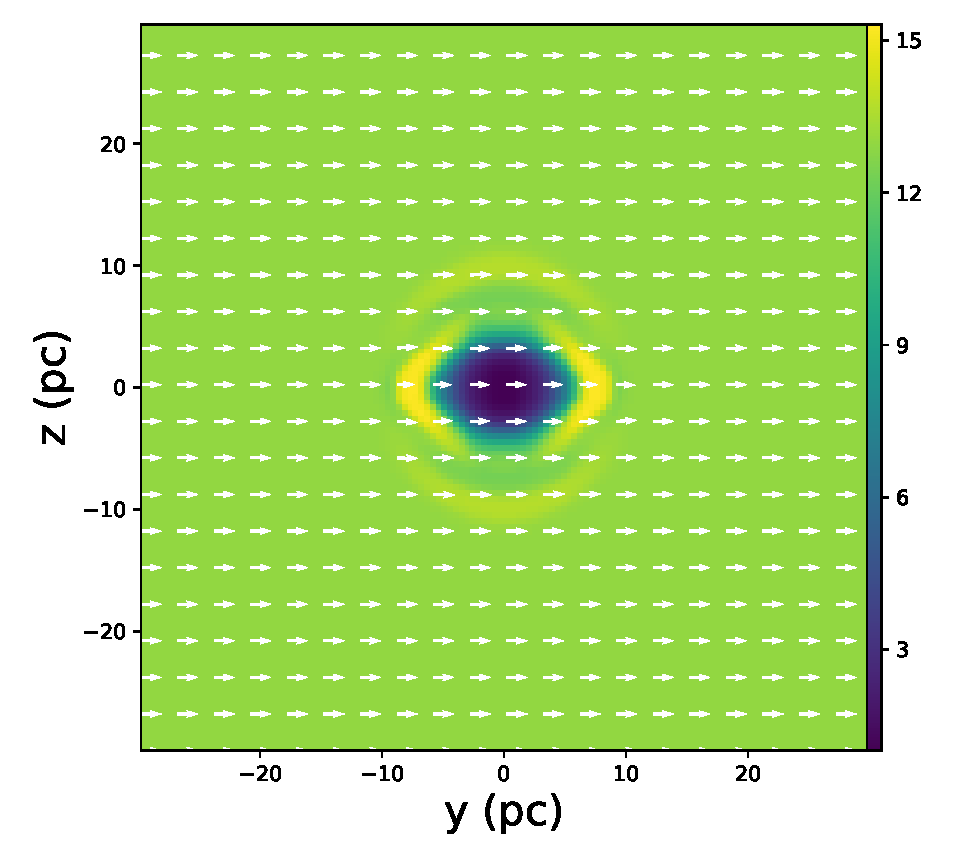
\includegraphics[width=0.475\textwidth]{rho_t20_density1_E1_yzR.eps}
    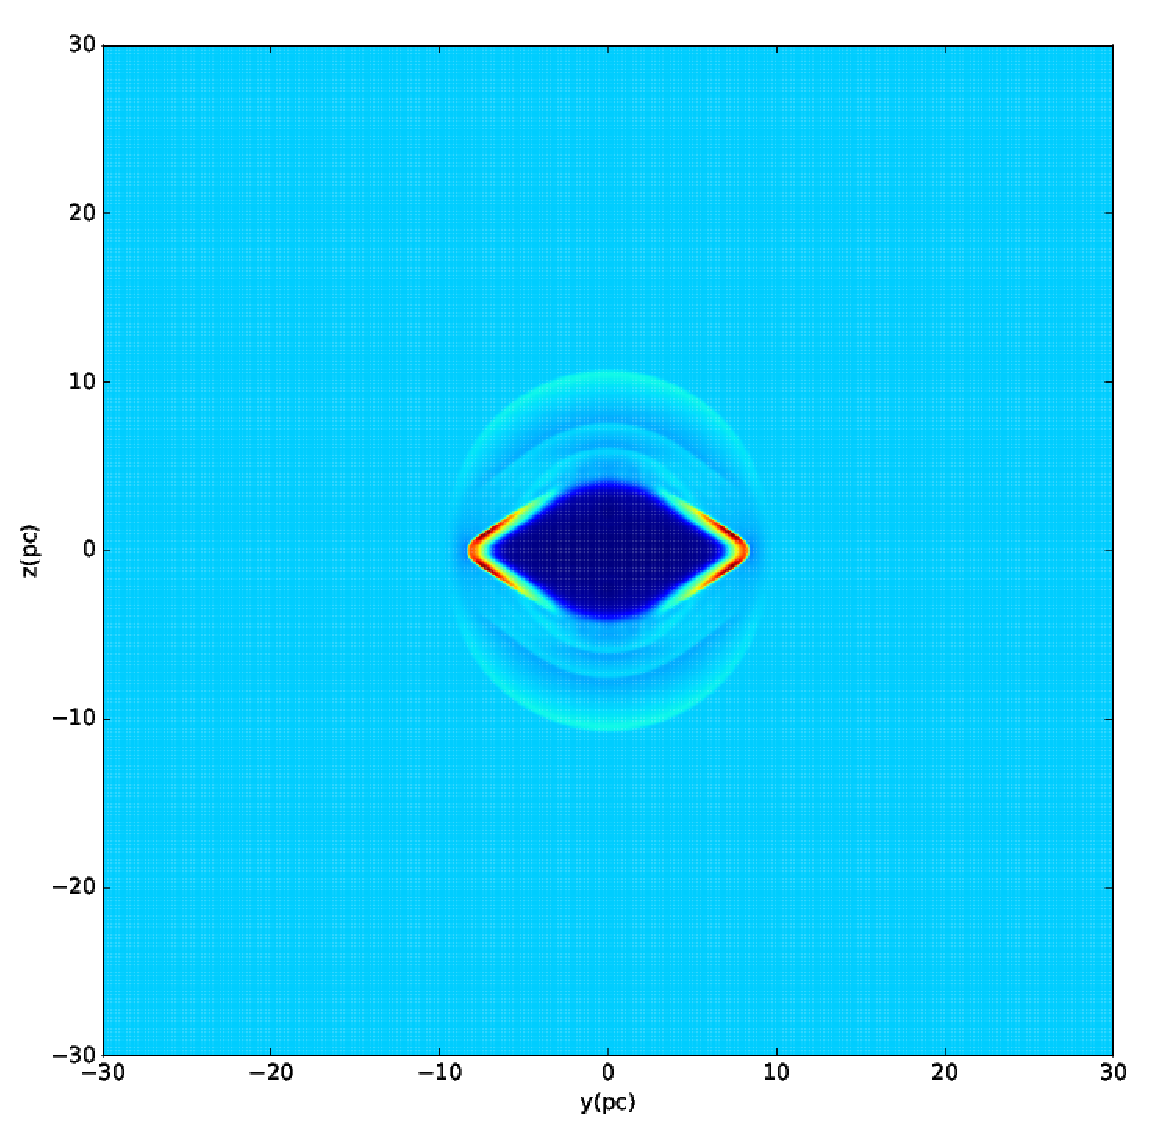
\includegraphics[width=0.435\textwidth]{10000_10.eps}
    \caption{介质密度为10 cm$^{-3}$的10000年演化结果。
    左图是低分辨率包含磁场方向的图像,右图是高分辨率真正出现多壳层的图像。}
\label{fig:shells}
\end{figure*}

\section{总结}
\label{MagSum}

我们在这一部分主要模拟了SNR在强磁场中的的演化,并得到了一些有用的信息:

\begin{enumerate}

    \item 强磁场中反向激波行为在不同方向存在很大差异,形成类似于喷流准直的现象。

    \item 这种准直现象在银河系中心或许会影响到费米泡的形成。

    \item 强磁场中演化的SNR也更有可能出现奇怪的射电和X射线图像,这或许可以解释
    G1.9+0.3的形态。

    \item 多壳层超新星遗迹在强磁场环境中容易出现,可实际形成机理与很多因素相关。

\end{enumerate}

要研究费米泡的形成,还需要大尺度又局部高分辨率的模拟,对计算性能要求很高。
另外,要解决G1.9+0.3的射电、X射线形态问题,以及多壳层的产生问题,需要调整多种参数
组合做测试,同样需要大量工作。
